\chapter{The Solow Model}\label{chp:solo}
\hypertarget{solow}{}

%No extra line here.
\textbf{Tools:} Capital accumulation dynamics; Cobb-Douglas production function.

\textbf{Key Words:} Investment; saving; depreciation; steady state; convergence.

\needspace{4\baselineskip}
\textbf{Big Ideas:}
%\vspace{-0.1in}
\begin{itemize}
    \item The Solow model connects saving and investment with economic growth.
    \item In the Solow model without productivity (TFP) growth, capital accumulation does not generate long-run growth. The reason is diminishing returns to capital: the impact of additional capital declines the more you have.  As a result, differences in saving rates have only modest effects on output per worker and none at all on its long-run growth rate.
    \item TFP growth generates long-run growth in output per worker.
\end{itemize}

\rule{\textwidth}{1pt}

We see large differences in saving and investment rates across
countries, with (for example) the US investing 20 percent of GDP,
China 40 percent, and India 30 percent in recent years
(ratios of real investment to real GDP from the Penn World Tables).
How important are these differences to the growth rates of countries?
The answer:  not important at all.
Why?  Because diminishing returns to capital means
(in practice) that additional capital generates smaller and smaller
additions to output.
This insight comes from work by Robert Solow,
who received the 1987 Nobel Prize in economics for his work.
His model is also a useful tool for extrapolating current trends
and pointing out the critical inputs to any such exercise.


\section{The model}
%
Solow's model has four relatively simple components. \index{Solow, Robert}
The first is our friend the production function:\index{Solow model|(}
\begin{equation}
    Y_t \;\;=\;\; A_tF(K_t,L_t) \;=\; A_t K_t^{\alpha} L_t^{1-\alpha}.
        \label{eq:pf_solow}
\end{equation}
Changes in output, therefore, come from changes in
(total factor) productivity, capital, and/or labor.
Recall that one of the properties of this production function
is diminishing returns to capital --- each additional unit of capital leads to a smaller addition to output.
This is the critical ingredient in what follows.
The second component is a link between investment and saving.
You'll recall that the flow identity,
$  S = I + \NX $,
linked saving to investment and net exports.
Solow ruled out the last one (we can put it back later if we like),
giving us
\[
    S_t \;\;=\;\; I_t.
\]
Lurking behind the scenes here is the expenditure identity,
$ Y = C + I$ in this case.

The third component is a description of saving behavior:
people save a constant fraction $s$ of their income,
\[
    S_t \;\;=\;\; sY_t,
\]
where the saving rate $s$ is a number between zero and one.
This is a little simplistic --- you might expect saving to depend on
the rate of return and/or expectations of future income --- but there is a lot to be said for simplicity.
For our purposes, $s$ is really the investment rate (the ratio of
investment to GDP), but since saving and investment are the same
here, we can call it the saving rate.
Finally, the capital stock depreciates at a constant rate $\delta$,
so that
\begin{eqnarray}
    K_{t+1} &=& (1-\delta) K_t + I_t ,
    \label{eq:k}
\end{eqnarray}
where the depreciation rate $\delta$ is a number between zero and one.


The model consists of these four equations.
This seems kind of simple for a Nobel Prize, but they really are good equations.
Now let's see where they lead.


\section{Capital dynamics}
%
Let's think about how the model behaves if the labor input $L$
and productivity $A$ are constant.
Analysis of the model in this case consists of describing
how the capital stock evolves through time.
Other variables follow from their relations to the capital stock.
We can find output from the production function,
saving (= investment) from output,
and consumption (should we need it) from the expenditure identity ($ C = Y - I$).

The key step is to describe how the capital stock changes from one period to the next.
To do that, we add time subscripts to the equations that don't have them already.
Then, with a little work, we see that the capital stock behaves like this:
\begin{eqnarray}
    K_{t+1} &=& (1-\delta) K_t + I_t \nonumber \\
            &=& (1-\delta) K_t + S_t \nonumber  \\
            &=& (1-\delta) K_t + s Y_t \nonumber \\
            &=& (1-\delta) K_t + s A K_t^\alpha L^{1-\alpha} .
            \label{eq:k-lom}
\end{eqnarray}
Note that each step follows from one of the components of the model.
The result is a formula for computing $K_{t+1}$ from $K_t$ and some other stuff.
%For practice, you
If we have numerical values for the parameters $(A,\alpha,s,\delta)$,
we can do the computations in a spreadsheet or other program
and see how $K$ moves through time.


\textbf{Example.} A numerical example will show you how this works.
Let $L = 100$, $ A = 1$, $s = 0.2$, $\delta = 0.1$, and $\alpha =
1/3$. (We'll use the same parameters throughout.) If the initial
capital stock is 250, we can compute future values of the capital
stock by applying equation (\ref{eq:k-lom}) repeatedly.
We then compute output from the capital
stock using the production function. The results for this case are
summarized in Table~\ref{tab:example}.
%
\tabcolsep = 0.1in
\begin{table}[t]
\centering
\caption{Output dynamics in the Solow model.}
\begin{tabular}{ccc}
\toprule
Date $t$  &  Capital Stock $K$ &  Output $Y$ \\
\midrule
    0 & 250.0 & 135.7 \\
    1 & 252.1 & 136.1 \\
    2 & 254.2 & 136.5 \\
    3 & 256.0 & 136.8 \\
    4 & 257.8 & 137.1 \\
    5 & 259.4 & 137.4 \\
    6 & 261.0 & 137.7 \\
    7 & 262.4 & 137.9 \\
    8 & 263.8 & 138.2 \\
    9 & 265.0 & 138.4 \\
   10\phantom{0} & 266.2 & 138.6 \\
%   11 & 267.2864 & 138.7796 \\
%   12 & 268.3136 & 138.9572 \\
%   13 & 269.2737 & 139.1227 \\
%   14 & 270.1709 & 139.2770 \\
%   15 & 271.0092 & 139.4209 \\
%   16 & 271.7925 & 139.5551 \\
%   17 & 272.5242 & 139.6803 \\
%   18 & 273.2079 & 139.7970 \\
%   19 & 273.8465 & 139.9058 \\
%   20 & 274.4430 & 140.0073 \\
\bottomrule
\end{tabular}
\label{tab:example}
\end{table}
%
[Suggestion:  Try to reproduce a few periods of the table to
make sure you understand how it works.
If you get stuck, read the last two pages again.
The trick is to set up formulas that tie each period to the previous one.]


You can see in the table
that capital and output both increase over time.
Will they increase forever?
The answer is no, but it takes a little work to
show. (Alternatively, you could extend the simulation and see what
happens.)
This is an important conclusion, because it tells us saving
and capital formation can't be the reason
(in this model, anyway)
that some countries grow faster than others.  More on this soon.


The dynamics of the capital stock reflect a balance of two factors:
(i)~saving tends to increase the capital stock by financing new investment
and (ii)~depreciation tends to reduce it.
A modest change to equation (\ref{eq:k-lom}) makes this clear:
\begin{eqnarray}
    \Delta K_{t+1} &\equiv& K_{t+1} - K_t
            \;\;=\;\;  s A K_t^\alpha L^{1-\alpha} - \delta K_t .
            \label{eq:dK}
\end{eqnarray}
(The equal sign with three lines means that the equation defines
the expression that comes before it, in this case $\Delta K_{t+1}$.)
You can see that the change is zero (the capital stock doesn't change)
when
\[
    K_{ss} \;\;=\;\; \left( \frac{s A}{\delta} \right)^{1/(1-\alpha)} L ,
\]
where $K_{ss}$ is the ``steady-state'' capital stock.
This is a little complicated, but remember:  it's just a formula.
In our example, $K_{ss} = 282.8$, so we have a ways to go before the model reaches
its steady state.
\begin{figure}[ht]
    \caption{The Solow model.}
    \centering
    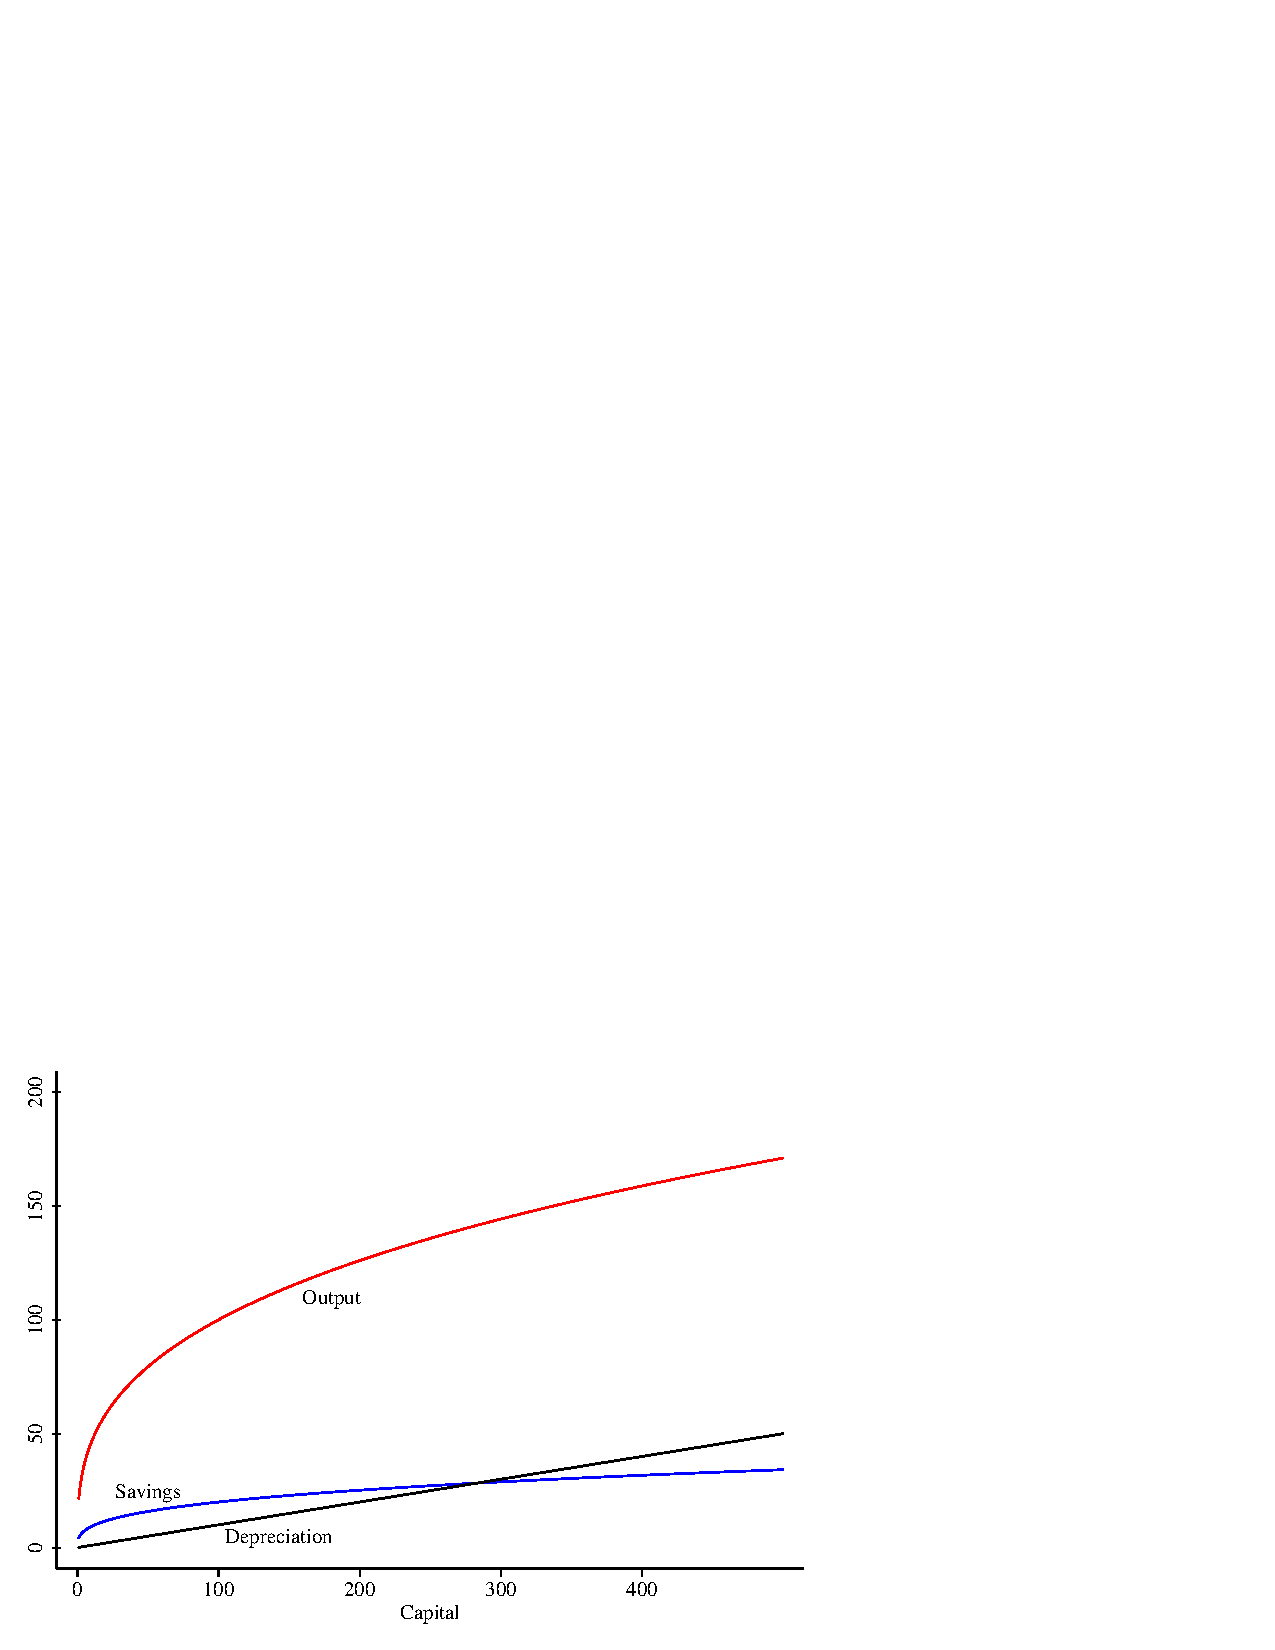
\includegraphics[width=0.8\textwidth]{\figpath Figures/solow1.pdf}\\
    \label{fig:solow1}
\end{figure}

What happens if we are above or below $K_{ss}$?
You can get a sense of the dynamics from Figure~\ref{fig:solow1}.
The top line is output,
which is related to the capital stock through the production function.
The next line is saving, a constant fraction of output
and the first expression on the right side of equation (\ref{eq:dK}):  $s A K^\alpha L^{1-\alpha} $.
The third line is depreciation, a constant fraction $\delta$
of the capital stock and the second object on the right side of equation (\ref{eq:dK}):  $\delta K $.
Diminishing returns to capital gives the saving line its curvature.
It leads to higher saving than depreciation at low
values of the capital stock, so the capital stock is increasing.
Similarly, saving is lower than depreciation at high values of the capital stock,
so the capital stock falls.
The crossing point is $K_{ss}$, where saving is just enough to
make up for depreciation, leaving the capital stock unchanged.


\section{Convergence\index{Solow model!convergence}}

The central feature of the model is what we call the convergence property:
If countries have the same parameters, they will eventually converge to the same
level of output per worker.
We haven't quite shown this yet, but the only thing missing
is the ``per worker'' qualification.


Consider, then, a version of the model in per-worker terms.
The first step is to divide both sides of (\ref{eq:k-lom}) by $L$.
If $k \equiv K/L$ is capital per worker (or the capital-labor ratio), the equation becomes
\begin{eqnarray*}
   k_{t+1} &=& (1-\delta) k_t + s A k_{t}^{\alpha}
\end{eqnarray*}
or
\begin{eqnarray}
   \Delta k_{t+1} &\equiv& k_{t+1} - k_t
            \;\;=\;\; s A k_{t}^{\alpha} - \delta k_t  .
   \label{eq:dk}
\end{eqnarray}
You'll note a resemblance to equation (\ref{eq:dK}).

Figure~\ref{fig:solow2} illustrates the model's dynamics.
It's based on the same parameter values as our earlier example:
$ A = 1$, $s = 0.2$, $\delta = 0.1$, and $\alpha = 1/3$.
\begin{figure}[ht]
\caption{The impact of the saving rate in the Solow model.}
    \label{fig:solow2}
    \centering
    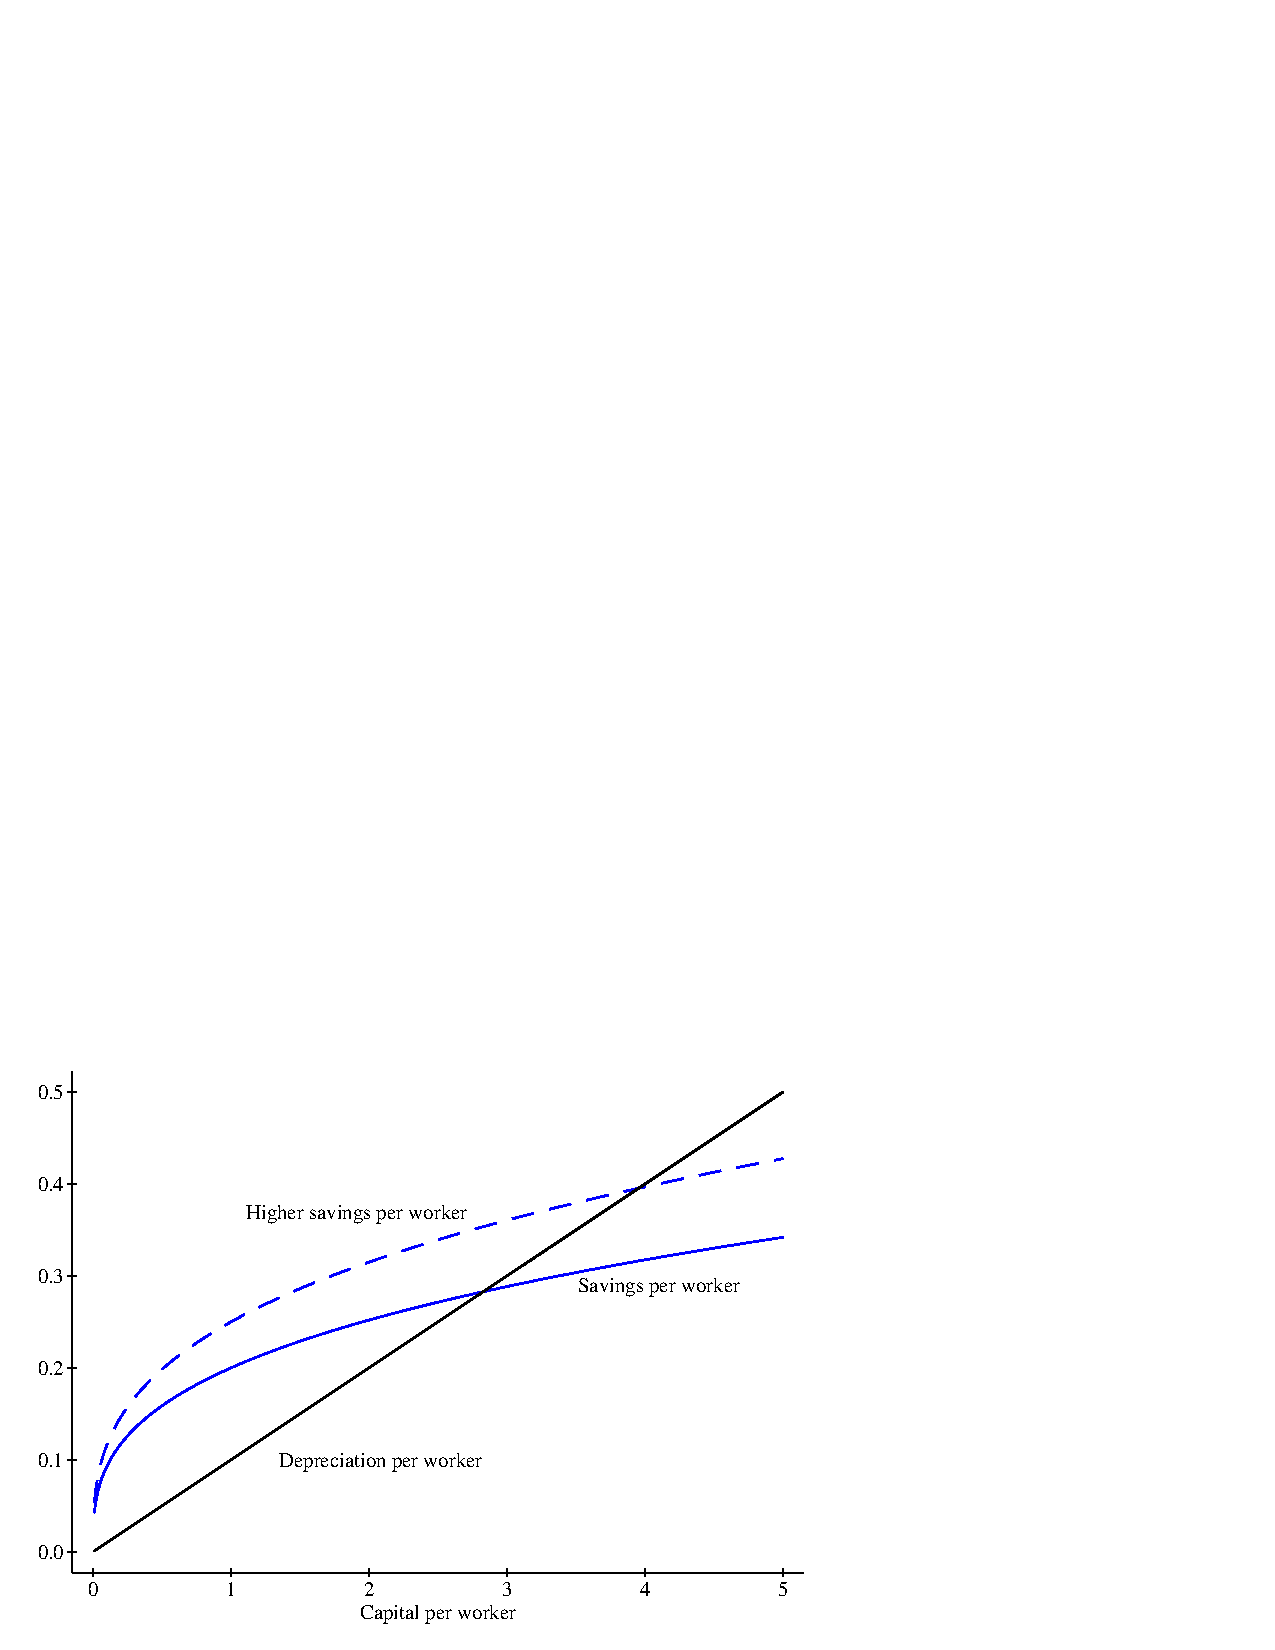
\includegraphics[width=0.8\textwidth]{\figpath Figures/solow2.pdf}\\
\end{figure}
The line marked ``saving per worker'' is the first expression on
the right side of equation (\ref{eq:dk}):  $ s A k^\alpha $. The
line marked ``depreciation per worker'' is the second expression
on the right side of equation (\ref{eq:dk}):  $\delta k$. For
small values of $k$, saving per worker is greater than
depreciation per worker, so $k$ increases. For large values of
$k$, saving per worker is less than depreciation per worker, so
$k$ decreases. The two lines cross at the steady state, where the
capital-labor ratio is constant. We can find the steady-state
value of $k$ from equation (\ref{eq:dk}) by setting $\Delta
k_{t+1} = 0$.  This leads to
\[
    k_{ss} \;=\; \left( \frac{sA}{\delta} \right)^{1/(1-\alpha)} ,
\]
a minor variant of our earlier expression for the steady-state capital stock.


We have shown that the capital-labor ratio eventually converges to its steady-state value.
What about output per worker?
The production function in per worker form is $ Y/L = A k^\alpha$,
so steady-state output per worker depends on steady-state capital per worker:
\begin{equation}
    (Y/L)_{ss}  \;\;=\;\; A k_{ss}^\alpha
                \;\;=\;\; A \left( \frac{sA}{\delta} \right)^{\alpha/(1-\alpha)}
                \;\;=\;\; A^{1/(1-\alpha)} \left( \frac{s}{\delta}
                \right)^{\alpha/(1-\alpha)} .
                \label{eq:ss-yl}
\end{equation}
Similarly, the steady-state capital-output ratio is
\[
    (K/Y)_{ss} \;\;=\;\; \left( \frac{s}{\delta} \right) .
\]
The algebra isn't pretty, but it tells us how the steady state
depends on the various parameters.
The last equation tells us, for example, that countries with higher saving rates
also have higher steady-state capital-output ratios --- that is more saving leads to more capital.
Equally important, the existence
of a steady state tells us that if two countries have the same
parameter values, they will converge to the same output per
worker. We refer to this as the convergence   property. In this
model, any long-term differences between countries must come from
differences in their parameters.


\section{Impact of saving \index{saving} and investment}

We can return to the question we began with: What is the impact of saving
and investment rates on growth and income?
The long-run impact of saving \index{saving}
on growth is zero;
the steady-state growth rate is zero, regardless of the saving rate.
But there is an effect of saving on steady-state output per worker.

Consider our example.
From equation (\ref{eq:ss-yl}), we see that steady-state
output per worker is 1.4142.
What if we increase the saving rate $s$ from 20 percent to 25 percent?
Then, steady-state output rises to 1.5811, an 11 percent increase.
This isn't irrelevant, but it's a relatively modest increase
for a substantial increase in saving.
It clearly does not explain much of the enormous differences
in GDP per capita that we see around the world.

We can see the same thing in Figure~\ref{fig:solow2}. The line marked
``saving per worker'' is based on a saving rate of $s = 0.20$, or
20 percent. If we raise the saving rate to  25 percent,
the saving line shifts up, as
shown by the dashed line marked ``higher saving per worker.'' Why?
Because $s A k^\alpha $ is higher at every value of $k$. With this
new line, the steady-state value of capital per worker (where the
saving line crosses the depreciation line) is higher, as shown.\index{Solow model|)}


\section{Growth}

If saving doesn't generate growth, what does?
We add growth in the labor force and
(critically) growth in total factor productivity
with two goals in mind.
The first goal is to account for the growth rate of output,
showing how it depends on the growth rates of our two inputs.
The second is to show that the economy approaches
what we call a balanced growth path in which
output and capital grow at the same rate.
As before, the capital-output ratio approaches a constant,
the features of which we can easily summarize.
We do this with a striking example in mind:
We know that China invests an astounding 40 percent of its GDP.
Is this too much?
A hint is that capital intensity
(measured by the capital-output ratio)
depends not only on the investment rate (which tells us how
much new capital is added), but also on the growth rate
(how fast the denominator is changing).
A fast-growing economy needs a high investment rate
simply to maintain a given capital-output ratio.


The new inputs into our analysis are growth in the   labor force \index{labor!labor force}
and productivity.
Let us say, to be concrete,
that labor and productivity grow
at constant rates:
\begin{eqnarray*}
    L_{t+1} &=&  (1+g_l) L_t \\
    A_{t+1} &=&  (1+g_a) A_t .
\end{eqnarray*}
How fast do output and capital grow?
Let's guess that output and capital grow at the same rate $g_y$,
to be determined.
(Why?  Because we're good guessers.)
From the production function, we then know that
\begin{eqnarray*}
    (1+g_y)       &=& Y_{t+1}/Y_t  \\
                &=&  (A_{t+1}/A_t) (K_{t+1}/K_t)^\alpha
                        (L_{t+1}/L_t)^{1-\alpha} \\
                &=& (1+g_a) (1+g_y)^{\alpha} (1+g_l)^{1-\alpha} .
\end{eqnarray*}
The growth rate, is therefore,
\begin{eqnarray*}
    (1+g_y)       &=& (1+g_a)^{1/(1-\alpha)} (1+g_l) .
\end{eqnarray*}
Just a formula, but it says that output growth is tied
to the growth rates of productivity and labor.
The saving rate does not affect this growth rate.
Similarly, the growth rate in output per worker is
\begin{eqnarray*}
    (1+g_y)/(1+g_l)     &=& (1+g_a)^{1/(1-\alpha)} ,
\end{eqnarray*}
which depends only on productivity growth.
If $\alpha$ is positive,
the growth rate of output per worker is
higher than the growth rate of productivity,
because the exponent $ 1/(1-\alpha)$ is greater than one.
In words, the direct impact of productivity on output
is magnified by the growth in the stock of capital;
see the production function (\ref{eq:pf_solow}).
This ties in with a remark we made earlier: That capital accumulation
tends to reinforce the impact of productivity growth.
Countries with high productivity also have a lot of capital.


What about capital --- do countries with higher saving rates have more
capital, relative to the size of their economies?
Consider, again, a steady state in which capital and output grow
at the same rate $g_y$.
Then $K_{t+1} = (1+g_y) K_t$ and equation (\ref{eq:k-lom}) becomes
\begin{eqnarray*}
    K_{t+1}  &=& (1-\delta) K_t + s Y_t  \\
    (1+g_y) (K_{t}/Y_{t}) &=& (1-\delta) (K_t/Y_t) + s .
\end{eqnarray*}
Solving for $K/Y$ gives us the steady-state capital-output ratio:
\begin{eqnarray*}
    (K/Y)_{ss} &=& \left( \frac{s}{\delta+g_y} \right) .
\end{eqnarray*}
%This line of argument doesn't actually require the Solow model.
%If we divide equation (\ref{eq:k-lom})
%by $Y_t$ and substitute $ Y_{t} =  Y_{t+1}/(1+g)$, we get
%\begin{eqnarray*}
%    (1+g) K_{t+1}/Y_{t+1}  &=& (1-\delta) K_t/Y_t + s .
%\end{eqnarray*}
%The steady state capital-output ratio
%(the ratio that makes $K_{t+1}/Y_{t+1}$ and $K_{t}/Y_{t}$ equal)
%is exactly what we just derived.

To return to our goal of understanding the sources of capital intensity,
note the impact of growth on the steady-state capital-output ratio.
For a given saving/investment rate $s$, countries with higher growth $g_y$
will have relatively less capital per unit of output.
Why?  Because when output is growing quickly,
you need to invest a lot to keep capital growing at the same rate.


\textbf{Example.}
Here are some numbers based loosely on the US:
$ g_l = 0.005 $ (0.5\%), $ g_a = 0.01 $ (1\%), $s=0.15$,
and $\delta = 0.06$.
What is the growth rate of output?
The steady-state capital-output ratio?
The growth rate satisfies
\[
    1+g_y \;\;=\;\; (1+g_a)^{1/(1-\alpha)} (1+g_l) \;\;=\;\; 1.015 \times 1.005
        \;\;=\;\; 1.0201.
\]
Here, we've used $\alpha = 1/3$, as usual.
Using the same parameters as our earlier examples, the steady-state
capital-output ratio is
\[
    1.872 \;\;=\;\; \frac{0.15}{0.06 + 0.020} .
\]
Now consider numbers based on China.
We keep $ g_l = 0.005 $ and $\delta = 0.06$,
but change the others to $ g_a = 0.05 $ and $s = 0.40 $.
The growth rate is now $g_y = 0.0813$ and the capital-output ratio
is 2.83. Note the moderate increase, despite the near tripling of the
saving/investment rate. Is China investing too much?
Perhaps not. Their capital-output ratio (by this calculation)
is not much different from that of the US, so the 40\% investment
rate isn't delivering excessive capital intensity by this measure.
They need to invest a lot simply to keep up with the growth
of their economy.


%\subsubsection*{Discussion}


%[??] Solow's work focussed attention on saving and investment.
%If high per capita income required high saving, then maybe we should save more.
%And if it required investment, poor countries should think about
%financing investment through foreign borrowing as well as domestic saving.
%Our sense is that neither of these conclusions are supported by the evidence.
%High saving rates do finance greater investment,
%but they come at the cost of lower consumption rates.
%And poor countries, as we'll see, are poor primarily because they
%have low productivity, not because they lack capital.


\section*{Executive summary}

%\setlength{\leftmargini}{.5\oldleftmargini}
\begin{enumerate}
\item Solow's model bases growth on saving and investment.

\item Saving affects steady-state GDP per worker,
but not its growth rate.
In this sense and others, saving is secondary to long-term
economic performance.

\item
%The steady state capital-output ratio depends
%on both the saving rate and the growth rate of the economy.
Fast-growing countries must invest more to maintain the same
capital-output ratio.
\end{enumerate}
%\setlength{\leftmargini}{\oldleftmargini}

\section*{Review questions}

%\setlength{\leftmargini}{.5\oldleftmargini}
\begin{enumerate}

\item The basics.  Suppose $A=L=K=1$, $\alpha = 1/3$, $\delta = 0.06$, and $s = 0.12$.
\begin{enumerate}
\item What is output $Y$?
\item What are saving $S$ and investment $I$?
\item What is next period's capital stock?
\end{enumerate}

\needspace{4\baselineskip}
Answer.
\begin{enumerate}
\item $Y = A K^{1/3} L^{2/3} = 1$.
\item $S=I = s Y = 0.12$.
\item Put $t$'s on everything so far.
Then $K_{t+1} = (1-\delta) K_t + I = 0.94 + 0.12 = 1.06$.
\end{enumerate}


\item Example, continued.  For the numerical example in the text:
\begin{enumerate}
\item Suppose that the economy starts with the steady-state capital stock.
What are the steady-state levels of output, investment, and consumption?
\item If 25 percent of the capital stock is destroyed in a war,
how long does it take the economy to eliminate half the fall in output?
\end{enumerate}

\needspace{4\baselineskip}
Answer.
\begin{enumerate}
\item The steady-state capital stock is (as we've seen) $K_{ss} = 282.8$.
Using this value, the production function tells us that output is 141.4.
Investment equals the depreciation of the capital stock, 28.3.
We can find consumption in two ways.
The first is through the expenditure identity:  $Y = C + I$.
We know $Y$ and $I$, so $C$ is 113.1.
The second is through the flow identity.
Saving is fraction $s$ of output, so consumption is fraction $1-s$,
$ 0.8 \times 141.4 = 113.1 $.
\item This requires a simulation.
Let the capital stock fall to 212.1, 75 percent of its steady-state value.
Then, output is 128.5, 90.9 percent of its steady-state value.
We recover half the fall if output rises to 135.0.
If we simulate the model, we see that it reaches 135.1 in 10 periods (years).
\end{enumerate}

\item Government.  We've ignored government so far.  Suppose, instead,
that the government purchases goods and services
equal to a constant fraction of GDP
(say, $ G = d Y$ for some fraction $d$)
 and collects taxes equal to the same fraction of output.
Individuals have after-tax income of $ (1-d) Y$ and save a
fraction $s$ of it.
With these changes, how would the analysis of the basic Solow model change?

Answer.  The critical ingredient here is the fraction of output allocated
to investment.
Investment here is $ I = S = s (1-d) Y $.
Effectively, $d$ reduces the saving rate from $s$ to $s(1-d)$
and takes resources away from investment.
If the government invests, we'd have to include that,
but we'd also have to decide how useful the investment was
(does it count the same as other investment?).

\begin{comment}
% ?? answer needs help
\item Population growth.
Consider the model with population growth, and suppose
that $\delta = 0.1$, $s = 0.2$, $A = 1$, and $g_l = 0.01$. How much does
steady-state output per worker fall if $g_l$ rises to 0.02? \\
Warning:  This is moderately difficult.
You can't apply a formula from the text,
you need to work out the steady state on your own.

Answer.  In this case and others like it,
what's constant in a steady state is $K/Y$,
meaning $K$ and $Y$ grow at the same rate.
Call this rate $g$; it implies, for example,
$ Y_{t+1} = (1+g) Y_t$, and the same for $K_t$.
The critical inputs are the dynamics of capital and the production function.
Let's take them one at a time.

(i) Capital.  Consider the dynamics of
capital in a steady state.
We divide equation (\ref{eq:k}) by $Y_t = Y_{t+1}/(1+g)$ to get
\begin{eqnarray*}
    (1+g) (K_{t+1}/Y_{t+1}) &=& (1-\delta) (K_t/Y_t) + s.
\end{eqnarray*}
In a steady state where $K/Y$ is constant, we have
$ (g+\delta) (K/Y) = s $.

(ii) Production function.  Take the ratio of equation
(\ref{eq:pf_solow}) at date $t+1$ to the same equation at date $t$:
\begin{eqnarray*}
    (Y_{t+1}/Y_t) &=& (A_{t+1}/A_t) (K_{t+1}/K_t)^\alpha (L_{t+1}/L_t)^{1-\alpha} .
\end{eqnarray*}
Our assumptions about growth rates gives us
$ (1+g) = (1+g)^\alpha (1+g_l)^{1-\alpha} $,
or $ (1+g) = (1+g_l)$.
Returning to (i), we see that
$ K/Y = s/(g_l+\delta) $.

(iii) Output per worker.
The last step is to make the shift from $K/Y$ to $Y/L$.
We divide the production function by $K$, giving us
\begin{eqnarray*}
    (K/L)^{1-\alpha} &=& A (K/Y)
        \;\;\;\Rightarrow\;\;\;
        K/L \;\;=\;\; \left( \frac{ A s}{g_l + \delta} \right)^{1/(1-\alpha)}.
\end{eqnarray*}

Now we can do the calculations.
With $g_l=0.01$, steady-state output per worker is 1.348.
When $g_l=0.02$, it falls to 1.291, a drop of about 4 percent.
\end{comment}



\end{enumerate}
%\setlength{\leftmargini}{\oldleftmargini}

\section*{If you're looking for more}

This material is covered in many macroeconomics textbooks.
Our favorites are
\begin{itemize}
\item Tyler Cowen and Alex Tabarrok,
{\it Modern Principles: Macroeconomics\/}, ch 7.
\item N. Gregory Mankiw, {\it Macroeconomics (6th edition)\/}, chs 7-8.
\end{itemize}
Any editions will do, but the chapter numbers may vary.


Goldman Sachs has used the Solow model
(and some heroic assumptions about fundamentals) to forecast the importance of
the BRICs (Brazil, Russia, India, and China)
to the world economy in 50 years.
See
``\href{http://www.goldmansachs.com/korea/ideas/brics/99-dreaming.pdf}
{Dreaming with BRICs}.''
It's a good example of how assumptions about productivity, population growth, and education can be used to generate plausible scenarios for the sizes of economies in the distant future.
(The equations on their page 18 should look familiar.)
This doesn't make forecasting any less hazardous, but it tells you
what the critical inputs are.
The key one here, of course, is productivity growth.

\section*{Symbols used in this chapter}

\begin{table}[H]
\centering
\caption{Symbol table.}
\begin{tabular*}{0.95\textwidth}{l@{\extracolsep{\fill}}l}
\toprule
Symbol & Definition\\
\midrule
$Y$                            &Output (real GDP)\\
$A$                            &Total factor productivity (TFP)\\
$K$                            &Stock of physical capital  (plant and equipment)\\
$L$                            &Quantity of labor (number of people employed)\\
$F(K,L)$                    &Function of inputs K and L in production function\\
$\alpha$                     &Exponent of $K$ in Cobb-Douglas   production function \\
                            &(= capital share of income)\\
$S$                            &Saving\\
$I$                            &Investment\\
$C$                            &Consumption\\
$s$                         &    Saving rate as a percent of income $Y$\\
$\delta$                     &Rate of depreciation of physical capital \\
$\Delta K$                    &Change of $K$ ($=K_{t+1}-K_{t}$)\\
$K_{ss}$                    &Steady-state capital stock\\
$(K/Y)_{ss}$                &Steady-state capital-output ratio\\
$k$                         &Capital per worker, or capital-labor ratio ($=K/L$)\\
$g_y$                     &Discretely-compounded growth rate of $Y$\\
$g_l$                     &Discretely-compounded growth rate of $L$\\
$g_a$                     &Discretely-compounded growth rate of $A$\\
$d$                         &Government purchases as a share of output $(G/Y)$\\
\bottomrule
\end{tabular*}
\end{table}

